% ====================================================================
% graphite_ica_ch2_v4-08.tex — Chapter 2 (statistical thermodynamics of entropy and reversible heat)
%   출발점: base_ch2_v3.tex skeleton. 범위: graphite coin half-cell only.
%   주제: partition function -> occupation distribution -> S_config/S_vib/S_elec
%        -> entropy coefficient -> reversible heat.
%   상태: v4-08 independent build.
%   build: xelatex 2-pass (kotex).
% ====================================================================
\documentclass[11pt,a4paper]{article}
\usepackage[margin=22mm]{geometry}
\usepackage{kotex}
\setmonofont{D2Coding}[Scale=MatchLowercase]
\usepackage{amsmath,amssymb,mathtools,bm}
\usepackage{booktabs,longtable,array}
\usepackage{enumitem}
\usepackage{amsthm}
\usepackage{tikz}
\usetikzlibrary{arrows.meta,calc,positioning}
\usepackage{hyperref}
\usepackage{fancyhdr}
\usepackage{lastpage}
\usepackage{setspace}
\setstretch{1.12}
\setlength{\parskip}{0.45em}\setlength{\parindent}{0pt}\setlength{\headheight}{14pt}
\setlength{\emergencystretch}{2em}
\hypersetup{colorlinks=true, linkcolor=blue, urlcolor=blue, citecolor=blue,
  pdftitle={흑연 음극 dQ/dV — Chapter 2 (v4-08): 통계열역학 엔트로피와 가역 발열}}
\pagestyle{fancy}\fancyhf{}
\lhead{흑연 음극 $dQ/dV$ — Ch.2 (v4-08, 통계열역학 엔트로피)}\rhead{\thepage/\pageref{LastPage}}
\renewcommand{\headrulewidth}{0.4pt}
\newtheorem*{keybox}{핵심}
\newtheorem*{srcbox}{문헌 근거}
\newtheorem*{warnbox}{주의}
\newcommand{\dd}{\mathrm{d}}
\newcommand{\rxn}{\mathrm{rxn}}
\newcommand{\eq}{\mathrm{eq}}
\newcommand{\rev}{\mathrm{rev}}
\newcommand{\irr}{\mathrm{irr}}
\newcommand{\oc}{\mathrm{oc}}
\newcommand{\config}{\mathrm{config}}
\newcommand{\vib}{\mathrm{vib}}
\newcommand{\elec}{\mathrm{elec}}
\newcommand{\eff}{\mathrm{eff}}
\newcommand{\hys}{\mathrm{hys}}
\newcommand{\FD}{\mathrm{FD}}
\newcommand{\BE}{\mathrm{BE}}
\renewcommand{\theequation}{2.\arabic{equation}}
\renewcommand{\thesection}{2.\arabic{section}}
\title{\textbf{\LARGE Chapter 2}\\[0.35em]\Large 코인 하프셀 엔트로피 계수와 가역 발열의 통계열역학\\[0.2em]\large — 분배함수, 점유분포, 섞임 겹침, 그리고 $\dot Q_\rev=-IT\,\partial U_\oc/\partial T$ (v4-08)}
\author{}\date{}

\begin{document}
\maketitle

% ====================================================================
\section*{서 — 엔트로피 계수는 분포의 온도 미분이다}
\addcontentsline{toc}{section}{서}
% ====================================================================
Chapter 1 은 흑연 음극 코인 하프셀의 $\dd Q/\dd V$ 를 전이별 logistic 종과 중심 전위
$U_j(T)$ 로 세웠다. Chapter 2 의 역할은 그 같은 곡선을 다시 피팅하는 것이 아니라, 그 logistic 이
무엇의 분포인지와 그 분포가 왜 엔트로피 계수 $\partial U_\oc/\partial T$ 및 가역 발열
$\dot Q_\rev$ 를 만드는지를 닫는 것이다. 범위는 \textbf{전극 대 Li 금속의 코인 하프셀 단독}이다.
전셀 합성, 양극-음극 엔트로피 차, 팩 열수지는 여기서 다루지 않는다.

엔트로피는 미시상태 확률분포의 넓이다. 가역 발열은 전류가 일을 하는 동안 그 분포를 다른 SOC 의
분포로 재배열하는 데 필요한 열이다. 그러므로 하프셀 엔트로피 계수는 단순한 보정항이 아니라,
\[
\boxed{\;\text{partition function}\to\text{occupation distribution}\to
S_{\config},S_{\vib},S_{\elec}\to\frac{\partial U_\oc}{\partial T}\to\dot Q_\rev\;}
\]
라는 통계열역학 사슬의 관측량이다. Chapter 1 의 logistic 폭 $w=RT/F$ 는 수치 편의가 아니라
configurational entropy 가 전위축에 투영된 폭이다.

본 장이 사용할 최종 출구는 Bernardi, Pawlikowski, Newman 의 에너지 수지 \cite{bernardi1985} 에서 나온다:
\begin{equation}
\dot Q = I(U_\oc-V)-I\,T\,\frac{\partial U_\oc}{\partial T},\qquad
\boxed{\;\dot Q_\rev=-I\,T\,\frac{\partial U_\oc}{\partial T}=-\frac{I\,T}{F}\Delta S(x)\;}.
\label{eq:bernardi_v4}
\end{equation}
여기서 $I>0$ 방전 규약이면 첫 항은 과전압 소산이고 둘째 항은 부호가 바뀔 수 있는 가역열이다.
평형 전위와 반응 깁스 에너지가 $\Delta G=-F U_\oc$ 로 묶이므로
$\Delta S=F\,\partial U_\oc/\partial T$ 이다 \cite{newman,msmr_partI}. 아래의 모든 수식은 이 하프셀
평형 전위 규약으로 쓴다.

% ====================================================================
\section{격자기체 분배함수에서 Chapter 1 logistic 이 나온다}\label{sec:partition}
% ====================================================================
먼저 자리 하나를 본다. 비어 있는 상태의 에너지를 0, Li 가 점유한 상태의 에너지를 $\varepsilon_0$,
Li 의 전기화학퍼텐셜을 $\mu$ 라 두면, grand-canonical 단일 자리 분배함수는
\begin{equation}
Z_1=1+\exp[-\beta(\varepsilon_0-\mu)],\qquad \beta=(k_B T)^{-1}.
\label{eq:z1}
\end{equation}
점유수 $n\in\{0,1\}$ 의 평균은
\begin{equation}
\theta\equiv\langle n\rangle
=\frac{\exp[-\beta(\varepsilon_0-\mu)]}{1+\exp[-\beta(\varepsilon_0-\mu)]}
=\frac{1}{1+\exp[\beta(\varepsilon_0-\mu)]}.
\label{eq:fdsite}
\end{equation}
이는 전자 Fermi--Dirac 분포와 같은 수학 구조지만, 여기서는 한 격자 자리에 Li 가 하나만 들어갈 수 있다는
배타성에서 온다. Chapter 1 의 전이 진행률 $\xi$ 는 탈리튬화 방향으로 둔다. 곧 Li 점유율은
$\theta=1-\xi$ 이고, 전위가 중심 $U_j$ 에서 벗어날 때
\begin{equation}
\xi_{\eq,j}(V,T)=\frac{1}{1+\exp[-\sigma_j(V-U_j)/w_j]},\qquad
w_j=\frac{RT}{F},
\label{eq:ch1logistic}
\end{equation}
가 된다. $g_j=\partial\xi_j/\partial U=\xi_j(1-\xi_j)/w_j$ 는 Chapter 1 의 $\dd Q/\dd V$ 봉우리 모양이다.
따라서 logistic 은 경험적 sigmoid 가 아니라 격자기체 점유 확률의 전위 표현이다.

% ====================================================================
\section{분포에서 configurational entropy 를 직접 계산한다}\label{sec:config}
% ====================================================================
상호작용이 없으면 위의 두 상태 자리들이 독립이다. 평균장 상호작용을 넣으면 Bragg--Williams
정규용액 자유에너지 \cite{huggins1942,bazant2013}
\begin{equation}
g(\theta)=g_0+\Delta h^0\theta
  +RT\{\theta\ln\theta+(1-\theta)\ln(1-\theta)\}
  +\Omega\,\theta(1-\theta)
\label{eq:bw}
\end{equation}
가 된다. 괄호 안의 로그항은 분포의 조합수이고, $\Omega$ 는 서로 다른 이웃을 만들 때의 평균장 상호작용
에너지다. $\Omega>0$ 이 크면 분포는 넓게 섞이기보다 두 조성으로 나뉘려 하고, $\Omega\to2RT$ 에서
중심 기울기가 사라져 plateau 또는 상분리 한계가 나타난다.

자리 1몰의 Li 점유율을 $\theta$ 라 쓰면, 각 자리는 확률 $p_1=\theta$, $p_0=1-\theta$ 의 이항분포다.
Boltzmann--Shannon 엔트로피는
\begin{equation}
S_{\config}=-R\sum_i p_i\ln p_i
  =-R\{\theta\ln\theta+(1-\theta)\ln(1-\theta)\}.
\label{eq:sconfigtheta}
\end{equation}
이 식은 ``혼합 엔트로피''라는 이름으로 한 줄에 놓고 지나갈 항이 아니다. 식~\eqref{eq:z1} 의
분배함수에서 얻은 점유분포가 바로 식~\eqref{eq:sconfigtheta} 의 $p_i$ 를 정한다. 탈리튬화 진행률
$\xi=1-\theta$ 로 쓰면
\begin{equation}
S_{\config}(\xi)=-R\{(1-\xi)\ln(1-\xi)+\xi\ln\xi\},
\label{eq:sconfigxi}
\end{equation}
이고, Li 추출(탈리튬화) 진행률에 대한 부분몰 configurational entropy 는
\begin{equation}
\frac{\partial S_{\config}}{\partial \xi}
=R\ln\frac{1-\xi}{\xi}.
\label{eq:partialconfig}
\end{equation}
반대로 하프셀 전위식은 Chapter 1 규약에서
\begin{equation}
U_j(\xi,T)=U_j^0(T)+\frac{RT}{F}\ln\frac{\xi}{1-\xi}
\label{eq:singletransitionu}
\end{equation}
이므로, 고정 $\xi$ 에서
\begin{equation}
\frac{\partial U_j}{\partial T}\bigg|_{\xi}
=\frac{\partial U_j^0}{\partial T}+\frac{R}{F}\ln\frac{\xi}{1-\xi}
=\frac{1}{F}\left[\Delta S^0_{\rxn,j}+R\ln\frac{\xi}{1-\xi}\right].
\label{eq:singletransitiondudt}
\end{equation}
식~\eqref{eq:partialconfig} 와 식~\eqref{eq:singletransitiondudt} 의 로그 부호가 반대로 보이는 것은
어느 방향의 반응 엔트로피를 세는지의 차이다. 본 장의 $\Delta S(x)=F\partial U_\oc/\partial T$ 는
하프셀 전위의 온도 기울기 규약으로 정의하므로 식~\eqref{eq:singletransitiondudt} 를 따른다. 따라서
$\xi\to0$ 의 Li-rich 끝에서는 configurational 전위 엔트로피 계수가 $-\infty$, $\xi\to1$ 의 Li-poor 끝에서는
$+\infty$ 로 발산하며, $\xi=1/2$ 에서 0 이 되어 중심 표준값만 남는다.

\begin{keybox}
\textbf{이중계산 B.} $\Delta S^0_{\rxn,j}$ 는 $\xi=1/2$ 에서 정의한 전이 중심 표준값이다. 봉우리 내부
$R\ln[\xi/(1-\xi)]$ 항은 logistic 폭 $w=RT/F$ 가 이미 만든 configurational 항이다. 그러므로
$\Delta S^0_{\rxn,j}$ 에 config entropy 를 다시 넣으면 같은 분포를 두 번 더하는 오류가 된다.
\end{keybox}

\begin{figure}[t]
\centering
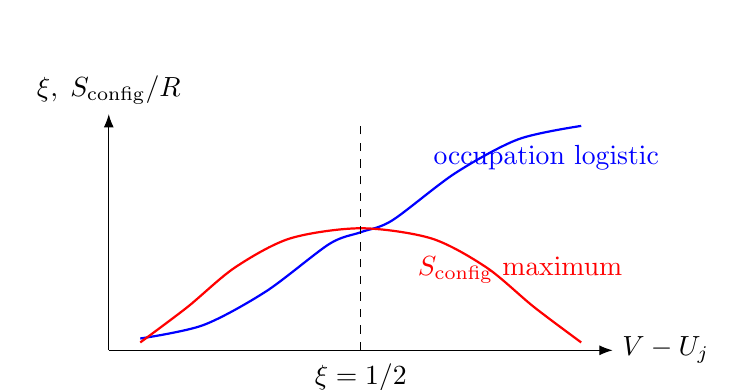
\begin{tikzpicture}[x=1cm,y=1cm,>=Latex]
  \draw[->] (0,0) -- (6.4,0) node[right] {$V-U_j$};
  \draw[->] (0,0) -- (0,3.0) node[above] {$\xi,\;S_{\config}/R$};
  \draw[thick,blue] plot[smooth] coordinates {
    (0.4,0.15) (1.2,0.32) (2.0,0.75) (2.8,1.35) (3.2,1.50)
    (3.6,1.65) (4.4,2.25) (5.2,2.68) (6.0,2.85)};
  \draw[thick,red] plot[smooth] coordinates {
    (0.4,0.10) (1.0,0.55) (1.6,1.05) (2.3,1.42) (3.2,1.55)
    (4.1,1.42) (4.8,1.05) (5.4,0.55) (6.0,0.10)};
  \draw[dashed] (3.2,0) -- (3.2,2.85);
  \node[blue,anchor=west] at (4.0,2.45) {occupation logistic};
  \node[red,anchor=west] at (3.8,1.02) {$S_{\config}$ maximum};
  \node[align=center] at (3.2,-0.35) {$\xi=1/2$};
\end{tikzpicture}
\caption{A single transition is a two-state lattice-gas distribution. The same distribution gives the logistic occupation and the configurational entropy maximum at $\xi=1/2$.}
\label{fig:distribution}
\end{figure}

% ====================================================================
\section{총 엔트로피는 config, vibrational, electronic 분포의 합이다}\label{sec:decomp}
% ====================================================================
단일 전이의 관측 엔트로피 계수는 중심 표준값, configurational 항, 그리고 분포 기반의 vibrational/electronic
항으로 나뉜다:
\begin{equation}
\boxed{\;
\Delta S_j(\xi,T)
=\Delta S^0_{\rxn,j}
R\ln\frac{\xi}{1-\xi}
\Delta S_{\vib,j}(\xi,T)
\Delta S_{\elec,j}(\xi,T)\;,\qquad
\frac{\partial U_j}{\partial T}=\frac{\Delta S_j}{F}.
}
\label{eq:decomp}
\end{equation}
$\Delta S^0_{\rxn,j}$ 는 전이 중심에서의 표준 반응 엔트로피다. 문헌상 흑연은 저 Li 분율에서 양의
부분몰 엔트로피, 고 Li 분율에서 음의 엔트로피를 보이며 \cite{reynier2003,allart2018}, Chapter 1 의
$+29,0,-5,-16$ J\,mol$^{-1}$K$^{-1}$ 입력은 그 부호와 규모를 따른다. 다만 식~\eqref{eq:decomp} 에서는
그 값들을 ``전이당 상수 함수''가 아니라 중심 표준값으로만 쓴다.

Vibrational entropy 는 포논의 Bose--Einstein 분포에서 온다. 진동 모드 $k$ 의 평균 점유수와 엔트로피는
\begin{equation}
n_k^{\BE}=\frac{1}{\exp(\beta\hbar\omega_k)-1},\qquad
S_{\vib}=R\sum_k\{(1+n_k)\ln(1+n_k)-n_k\ln n_k\}.
\label{eq:vib}
\end{equation}
Li 삽입으로 결합 강성, 층간 거리, stage 질서가 바뀌면 포논 스펙트럼 $\omega_k(x)$ 가 바뀐다. 흑연의
고 Li 영역에서 관측되는 음의 baseline 은 이 vibrational contribution 이 지배하는 것으로 해석된다
\cite{reynier2003,jpcc2021}. Chapter 2 의 피팅 식에서는 전이 폭 안에서 천천히 변하는 vib 항을
$\Delta S^0_{\rxn,j}$ 에 흡수하고, 빠른 변화가 보이는 경우에만 별도 $\xi$ 의존으로 남긴다.

Electronic entropy 는 전자의 Fermi--Dirac 분포에서 온다:
\begin{equation}
f(E)=\frac{1}{\exp[(E-E_F)/k_B T]+1},\qquad
S_{\elec}\simeq\frac{\pi^2}{3}k_B^2T\,g(E_F)
\label{eq:electronic}
\end{equation}
(Sommerfeld 한계). 흑연 하프셀에서는 대개 작지만, Ch1 v9 에서 확장한 LCO metal--insulator transition
사례처럼 $g(E_F)$ 가 급변하는 재료에서는 $\Delta S_{\elec}$ 가 관측 $\partial U/\partial T$ 에 들어간다.
삽입 기준 electronic entropy 변화는 음의 부호를 가질 수 있으며, 본 장의 흑연 중심 계산에서는 ``작거나
중심값에 흡수된 항''으로 취급한다.

% ====================================================================
\section{겹친 전이의 엔트로피 계수는 dQ/dV 비중으로 섞인다}\label{sec:overlap}
% ====================================================================
하프셀 OCV 는 여러 전이의 implicit sum 으로 정해진다:
\begin{equation}
\sum_j Q_j\,\xi_{\eq,j}(U_\oc,T)=Q_{\mathrm{tot}}\,x.
\label{eq:implicit}
\end{equation}
고정 $x$ 에서 미분하면
\begin{equation}
\frac{\partial U_\oc}{\partial T}\bigg|_x
=-\frac{\sum_j Q_j\,\partial\xi_j/\partial T|_U}
        {\sum_j Q_j\,\partial\xi_j/\partial U|_T}.
\label{eq:implicitdiff}
\end{equation}
$g_j=\partial\xi_j/\partial U=\xi_j(1-\xi_j)/w_j$ 를 쓰면, config 항을 분리한 중심값 가중식은
\begin{equation}
\boxed{\;
\frac{\partial U_\oc}{\partial T}
=\frac{1}{F}\,
\frac{\sum_j Q_j\,g_j\,\Delta S^0_{\rxn,j}}
     {\sum_j Q_j\,g_j}
\;}
\label{eq:overlapcenter}
\end{equation}
이다. 이 식의 의미는 명확하다. 전이 $j$ 의 entropy coefficient 는 그 전이가 현재 전압에서 얼마나
용량을 움직이는지, 즉 국소 $\dd Q/\dd V$ 비중 $Q_jg_j/\sum_k Q_kg_k$ 로 평균된다. 따라서 관측
$\partial U_\oc/\partial T$ 는 전이 경계에서 계단처럼 뛰지 않고, 겹친 봉우리 사이를 연속적으로 이동한다.

측정 전체를 재현하려면 config 항도 같은 비중으로 더한다. $z_j=(U_\oc-U_j)/w_j$ 라 두면 완전식은
\begin{equation}
\boxed{\;
\frac{\partial U_\oc}{\partial T}
=\frac{\sum_j Q_jg_j\left(\Delta S^0_{\rxn,j}/F+z_jR/F\right)}
       {\sum_j Q_jg_j}
\;}
\label{eq:overlapfull}
\end{equation}
이다. 제공된 수치검증에서는 Chapter 1 graphite staging 파라미터를 써서 $292.15$--$298.15$ K 유한차분
$\partial U_\oc/\partial T$ 와 식~\eqref{eq:overlapfull} 이 부동소수점 수준에서 일치했다. config 를 뺀
중심값 가중식~\eqref{eq:overlapcenter} 은 피크 중심값과 겹침 평균을 설명하지만, 전체 비선형에서는
최대 약 $0.184$ mV/K 의 체계적 차이를 남긴다. 이는 결함이 아니라 의도적으로 분리한 configurational
항의 크기다.

\begin{figure}[t]
\centering
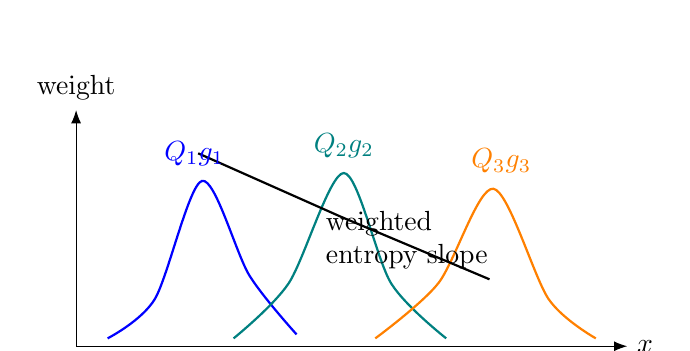
\begin{tikzpicture}[x=1cm,y=1cm,>=Latex]
  \draw[->] (0,0) -- (7.0,0) node[right] {$x$};
  \draw[->] (0,0) -- (0,3.0) node[above] {weight};
  \draw[thick,blue] plot[smooth] coordinates {(0.4,0.1) (1.0,0.6) (1.6,2.1) (2.2,0.9) (2.8,0.15)};
  \draw[thick,teal] plot[smooth] coordinates {(2.0,0.1) (2.7,0.8) (3.4,2.2) (4.0,0.8) (4.7,0.1)};
  \draw[thick,orange] plot[smooth] coordinates {(3.8,0.1) (4.6,0.8) (5.3,2.0) (6.0,0.6) (6.6,0.1)};
  \draw[thick,black] (1.55,2.45) -- (3.35,1.65) -- (5.25,0.85);
  \node[blue] at (1.5,2.45) {$Q_1g_1$};
  \node[teal] at (3.4,2.55) {$Q_2g_2$};
  \node[orange] at (5.4,2.35) {$Q_3g_3$};
  \node[align=left] at (4.2,1.35) {weighted\\entropy slope};
\end{tikzpicture}
\caption{Overlapping transitions blend entropy coefficients by local $\dd Q/\dd V$ weight, not by a step rule.}
\label{fig:overlap}
\end{figure}

% ====================================================================
\section{\texorpdfstring{$w_{\eff}(\Omega)$}{w eff Omega}, hysteresis, and limiting checks}\label{sec:limits}
% ====================================================================
정규용액 항 $\Omega$ 는 peak 폭과 entropy coefficient 를 함께 바꾼다. 중심 근방에서
\begin{equation}
\frac{\dd V_{\eq}}{\dd\xi}
=\frac{RT}{F}\left[\frac{1}{\xi(1-\xi)}-\frac{2\Omega}{RT}\right],
\qquad
\left.\frac{\dd V_{\eq}}{\dd\xi}\right|_{\xi=1/2}
=\frac{4RT-2\Omega}{F}.
\label{eq:regularslope}
\end{equation}
Chapter 1 logistic 폭과 같은 중심 기울기로 맞추면
\begin{equation}
\boxed{\;
w_{\eff}(\Omega)=\frac{w}{1-\Omega/(2RT)},\qquad \Omega<2RT.
\;}
\label{eq:weff}
\end{equation}
$\Omega\to2RT^-$ 에서 $w_{\eff}$ 가 발산한다. 이 한계는 넓고 평탄한 plateau 또는 상분리 임계에 대응하며,
단순한 넓은 Gaussian peak 가 아니다. $\Omega$ 자체가 온도 의존이면 $\partial w_{\eff}/\partial T$ 가
추가 entropy coefficient 를 만들지만, 흑연 코인 하프셀의 1차 모델에서는 중심 표준값과 config 항보다
작은 2차 항으로 둔다.

\begin{figure}[t]
\centering
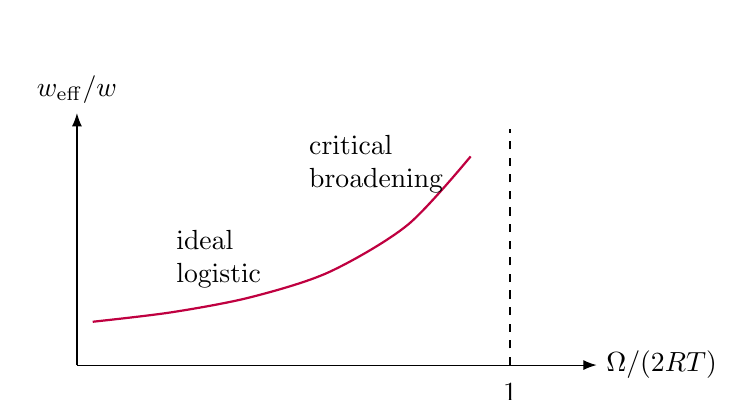
\begin{tikzpicture}[x=1cm,y=1cm,>=Latex]
  \draw[->] (0,0) -- (6.6,0) node[right] {$\Omega/(2RT)$};
  \draw[->] (0,0) -- (0,3.2) node[above] {$w_{\eff}/w$};
  \draw[thick,purple] plot[smooth] coordinates {
    (0.2,0.55) (1.2,0.67) (2.2,0.86) (3.2,1.18) (4.2,1.78) (5.0,2.65)};
  \draw[dashed] (5.5,0) -- (5.5,3.0);
  \node at (5.5,-0.35) {$1$};
  \node[align=left] at (3.8,2.55) {critical\\broadening};
  \node[align=left] at (1.8,1.35) {ideal\\logistic};
\end{tikzpicture}
\caption{Mean-field interaction changes the effective transition width. The formula is valid on the single-phase side $\Omega<2RT$.}
\label{fig:weff}
\end{figure}

Hysteresis must be separated from reversible entropy. Let branch $d\in\{\mathrm{ch},\mathrm{dis}\}$ have
branch centers
\begin{equation}
U_j^{(d)}(T)=U_j^0(T)\pm\frac{1}{2}\Delta U_j^{\hys}(T),
\qquad
g_j^{(d)}=\frac{\xi_j^{(d)}(1-\xi_j^{(d)})}{w_j^{(d)}}.
\label{eq:hyscenter}
\end{equation}
Then each branch has its own measured slope,
\begin{equation}
\frac{\partial U_\oc^{(d)}}{\partial T}
=\frac{1}{F}\frac{\sum_jQ_jg_j^{(d)}\Delta S^0_{\rxn,j}}
                 {\sum_jQ_jg_j^{(d)}}+\text{config/vib/electronic terms}.
\label{eq:hysbranch}
\end{equation}
The reversible coefficient used for $\dot Q_\rev$ is the branch average
\begin{equation}
\frac{\partial U^{\rev}}{\partial T}
=\frac{1}{2}\left(\frac{\partial U^{\mathrm{ch}}}{\partial T}
                 +\frac{\partial U^{\mathrm{dis}}}{\partial T}\right).
\label{eq:hysavg}
\end{equation}
The hysteresis gap itself gives irreversible heat proportional to $I\Delta U^{\hys}$ and must not be folded into
$\Delta S^0_{\rxn,j}$. Temperature dependence of the gap may be reported separately, but it is not the reversible
half-cell entropy coefficient.

\begin{table}[t]
\centering\small
\renewcommand{\arraystretch}{1.14}
\caption{Corner checks for the Ch2 v4 half-cell entropy model.}
\label{tab:limits}
\begin{tabular}{p{0.22\linewidth}p{0.36\linewidth}p{0.31\linewidth}}
\toprule
Limit & Behavior & Interpretation \\
\midrule
$\xi\to0$ & $R\ln[\xi/(1-\xi)]\to-\infty$ & Li-rich ordered end; config term dominates. \\
$\xi\to1$ & $R\ln[\xi/(1-\xi)]\to+\infty$ & Li-poor dilute end; large positive entropy slope. \\
$\xi=1/2$ & config term $=0$ & center standard $\Delta S^0_{\rxn,j}/F$ recovered. \\
$\Omega\to2RT^-$ & $w_{\eff}\to\infty$ & plateau/phase-separation critical limit. \\
single peak & weighted formula reduces to one transition & $\partial U/\partial T=\Delta S^0_j/F+$ config. \\
high $T$ electronic & $S_{\elec}\propto T\,g(E_F)$ & constant $\Delta S^0_j$ is safe only if $g(E_F)$ varies slowly. \\
\bottomrule
\end{tabular}
\end{table}

% ====================================================================
\section{코인 하프셀 데이터에서 \texorpdfstring{$\partial U/\partial T$ 와 $\dot Q_\rev$}{dU/dT and reversible heat} 를 산출한다}\label{sec:usable}
% ====================================================================
실험 사용 순서는 다음과 같이 닫힌다. 첫째, 낮은 전류 또는 휴지 충분한 코인 하프셀에서 여러 온도
$T_k$ 의 $U_\oc(x,T_k)$ 또는 준평형 $\dd Q/\dd V$ 를 얻는다. 둘째, Chapter 1 의 전이별 logistic/MSMR
구조로 모든 $T_k$ 를 동시에 맞추되 $U_j^0(T)$ 를 저차 온도 함수로 둔다 \cite{msmr_partI,msmr_partII}.
셋째, 전이 중심에서
\begin{equation}
\Delta S^0_{\rxn,j}=F\,\frac{\dd U_j^0}{\dd T}
\label{eq:fitcenter}
\end{equation}
를 얻고, SOC 별 관측값은 식~\eqref{eq:overlapfull} 로 재구성한다. 넷째, branch hysteresis 가 보이면
식~\eqref{eq:hysavg} 로 가역 평균을 만들고, gap 은 별도 비가역 항으로 둔다.

최종 가역 발열은
\begin{equation}
\boxed{\;
\dot Q_\rev(x,T,I)
=-I\,T\,\frac{\partial U_\oc}{\partial T}(x,T)
=-\frac{I\,T}{F}\Delta S(x,T).
\;}
\label{eq:qrevfinal}
\end{equation}
이 식은 열량계 보정식이 아니라 분포 재배열 열이다. $\partial U_\oc/\partial T>0$ 인 구간과 $<0$ 인 구간에서
같은 전류의 가역열 부호가 바뀌며, 전류 방향을 바꾸면 가역열도 반전한다. 과전압, ohmic drop, hysteresis
gap 으로 생기는 열은 $I(U_\oc-V)$ 또는 $I\Delta U^{\hys}$ 로 처리하며, 식~\eqref{eq:qrevfinal} 에 섞지 않는다.

\begin{warnbox}
\textbf{반응 엔트로피와 활성화 엔트로피는 다르다.} $\Delta S^0_{\rxn,j}=F\,\dd U_j^0/\dd T$ 는 평형 상태함수이고
가역열에 들어간다. Chapter 1 동역학 꼬리의 Eyring prefactor 에 들어가는 활성화 엔트로피는 비가역 속도
상수의 온도의존이다. 차원이 같아도 같은 항이 아니다.
\end{warnbox}

\begin{srcbox}
문헌 tier. Bernardi energy balance, Newman electrochemical thermodynamics, MSMR 온도 회귀는 직접 근거다
\cite{bernardi1985,newman,msmr_partI,msmr_partII}. 흑연 entropy profile 의 부호와 규모는
Reynier--Yazami--Fultz 및 Allart 등과 정합한다 \cite{reynier2003,allart2018}. Electrochimica Acta 2019
occupation 모델은 dilute 영역의 방법 선례로만 둔다 \cite{occupation2019}; 본 장의 전 범위 겹침식과
config 중복 금지 규칙은 Chapter 1 logistic 구조에서 유도한 working model 이다.
\end{srcbox}

% ====================================================================
\section*{맺음 — 가역열은 분포 재배열 열이다}
\addcontentsline{toc}{section}{맺음}
% ====================================================================
Chapter 2 의 핵심은 $U_j(T)$ 의 기울기를 표로 옮기는 데서 끝나지 않는다. 격자기체 분배함수는
Chapter 1 logistic 을 만들고, 그 점유분포는 $S_{\config}=-R\sum p\ln p$ 를 만들며, 포논과 전자 분포는
각각 $S_{\vib}$ 와 $S_{\elec}$ 를 더한다. 겹친 전이에서는 각 entropy coefficient 가 local $\dd Q/\dd V$
비중으로 섞이고, $\Omega$ 는 $w_{\eff}$ 를 통해 폭과 plateau 한계를 바꾸며, hysteresis gap 은 reversible
entropy 가 아니라 irreversible heat 로 분리된다. 따라서 코인 하프셀의 가역 발열
$\dot Q_\rev=-IT\,\partial U_\oc/\partial T$ 는 전극 내부 Li(+전자) 분포를 한 SOC 에서 다음 SOC 로
재배열하는 열이다.

% ====================================================================
\begin{thebibliography}{99}
\bibitem{bernardi1985} D. Bernardi, E. Pawlikowski, J. Newman, ``A General Energy Balance for Battery Systems,'' \emph{J. Electrochem. Soc.} \textbf{132}(1), 5--12 (1985). DOI: 10.1149/1.2113792.
\bibitem{newman} J. Newman, K. E. Thomas-Alyea, \emph{Electrochemical Systems}, 3rd ed., Wiley (2004). (OCV($T$): slope $=\Delta S$, intercept $=\Delta H$.)
\bibitem{reynier2003} Y. Reynier, R. Yazami, B. Fultz, ``The entropy and enthalpy of lithium intercalation into graphite,'' \emph{J. Power Sources} \textbf{119--121}, 850--855 (2003). DOI: 10.1016/S0378-7753(03)00285-4.
\bibitem{allart2018} D. Allart \emph{et al.}, ``Model of Lithium Intercalation into Graphite by Potentiometric Analysis with Equilibrium and Entropy Change Curves of the Graphite Electrode,'' \emph{J. Electrochem. Soc.} \textbf{165}(2), A380 (2018). DOI: 10.1149/2.1251802jes.
\bibitem{occupation2019} ``Transitions of lithium occupation in graphite: A physically informed model in the dilute lithium occupation limit supported by electrochemical and thermodynamic measurements,'' \emph{Electrochimica Acta} (2019). DOI: 10.1016/j.electacta.2019.135634. [방법 수준 인용 — 원문 식 미확보.]
\bibitem{chemmater2015} ``Intercalation Compounds from LiH and Graphite: Relative Stability of Metastable Stages\ldots,'' \emph{Chem. Mater.} \textbf{27} (2015). DOI: 10.1021/acs.chemmater.5b00235. [형성 ΔH calorimetry — abstract tier.]
\bibitem{jpcc2021} ``Thermodynamic Analysis of Li-Intercalated Graphite by First-Principles with Vibrational and Configurational Contributions,'' \emph{J. Phys. Chem. C} \textbf{125} (2021). DOI: 10.1021/acs.jpcc.1c08992. [abstract tier.]
\bibitem{msmr_partI} ``Quantifying the Entropy and Enthalpy of Insertion Materials for Battery Applications Via the Multi-Species, Multi-Reaction Model,'' \emph{J. Electrochem. Soc.} (2024). DOI: 10.1149/1945-7111/ad1d27.
\bibitem{msmr_partII} ``Quantifying the Temperature Dependence of the MSMR Model Part II: Estimation of Entropy Coefficient for Meso-Carbon Micro-Bead Graphite,'' \emph{J. Electrochem. Soc.} (2024). DOI: 10.1149/1945-7111/ad70d9.
\bibitem{standardised2024} ``A Standardised Potentiometric Method for the Effective Parameterisation of Reversible Heating in a Lithium-Ion Cell,'' \emph{J. Electrochem. Soc.} (2024). DOI: 10.1149/1945-7111/ad4918.
\bibitem{hysteresis2018} ``Uncertainties in entropy due to temperature path dependent voltage hysteresis in Li-ion cells,'' \emph{J. Power Sources} (2018). DOI: 10.1016/j.jpowsour.2018.05.060.
\bibitem{huggins1942} M. L. Huggins, ``Some Properties of Solutions of Long-chain Compounds,'' \emph{J. Phys. Chem.} \textbf{46}(1), 151--158 (1942). DOI: 10.1021/j150415a018.
\bibitem{bazant2013} M. Z. Bazant, ``Theory of Chemical Kinetics and Charge Transfer based on Nonequilibrium Thermodynamics,'' \emph{Acc. Chem. Res.} \textbf{46}(5), 1144--1160 (2013). DOI: 10.1021/ar300145c.
\end{thebibliography}

\end{document}
